\documentclass[conference]{IEEEtran}

\usepackage[utf8]{inputenc}
\usepackage[T1]{fontenc}
\usepackage{cite}
\usepackage{amsmath}
\usepackage{graphicx}
\usepackage{booktabs}
\usepackage{url}

\graphicspath{{../../outputs/figures/}}

\begin{document}

\title{Sentiment Classification of Reddit Comments with\\Dense, Recurrent and Transformer Models}

\author{
\IEEEauthorblockN{Nicolas Mejia, Daniel Barragan, Jacobo Rodriguez}
\IEEEauthorblockA{Computability and Data Structures III\\
Universidad Icesi, Cali, Colombia}
}

\maketitle

\begin{abstract}
We build a binary sentiment classifier (positive vs.\ negative) for short, informal Reddit
comments from the GoEmotions dataset. Each comment is labeled with the official mapping from
emotions to sentiment, and a balanced set of 1,000 comments is cleaned, split and vectorized
with a vocabulary learned only from the training data. A dense network, a vanilla RNN and an
LSTM are compared against a DummyClassifier baseline, and a pre-trained Transformer
(DistilBERT) is added as an extension. The architectures are also discussed in terms of
Turing machine concepts: memory, sequential processing and computability.
% TODO: add the final results (best model, accuracy, F1 and kappa on test) in one or two sentences.
\end{abstract}

\begin{IEEEkeywords}
sentiment analysis, GoEmotions, recurrent neural networks, LSTM, Transformer, Turing machines
\end{IEEEkeywords}

\section{Introduction}
\label{sec:introduction}

Sentiment analysis assigns a polarity to a piece of text. On social media this is harder than
on reviews or news: comments are short, informal and full of slang, emojis, sarcasm and
negations, and a single word such as ``not'' can reverse the meaning of the sentence. GoEmotions
\cite{demszky2020goemotions} is a corpus of English Reddit comments annotated with 27 emotions
plus neutral, together with an official grouping of the emotions into positive, negative and
ambiguous. In this work that grouping is used to turn the emotion labels into a binary
sentiment task (positive vs.\ negative).

The main objective is to compare three neural architectures that differ in how they handle
the order of the words and how much they remember: a dense network over word embeddings, which
has no memory of the sequence; a vanilla recurrent network (RNN) \cite{elman1990finding}, which
keeps a hidden state but suffers from vanishing gradients \cite{bengio1994learning}; and a Long
Short-Term Memory network (LSTM) \cite{hochreiter1997long}, whose gates control what is
written, kept and read from its memory cell. All of them share the same preprocessing and
vectorization, and they are compared with a DummyClassifier baseline using accuracy, precision,
recall, F1 and Cohen's kappa \cite{cohen1960coefficient}. As an extension we fine-tune
DistilBERT \cite{sanh2019distilbert}, a smaller version of BERT \cite{devlin2019bert} based on
the attention mechanism of the Transformer \cite{vaswani2017attention}.

A second objective is to relate these models to the theory of computation studied in the
course \cite{sipser2013introduction}. A recurrent network reads its input one symbol at a time
and updates a state, much like the transition function of an automaton; with unbounded
precision RNNs are Turing complete \cite{siegelmann1995computational}, and so are Transformers
\cite{perez2021attention}. Neural Turing Machines \cite{graves2014neural} make the analogy
explicit with an external memory and differentiable read and write heads. In practice, however,
every trained classifier performs a fixed number of operations per input and always halts, so
it decides a language of ``positive comments'' only approximately.

The rest of the report is organized as follows. Section~\ref{sec:data} describes the dataset,
the sentiment mapping and the preprocessing. Section~\ref{sec:models} presents the neural
architectures and their training, and Section~\ref{sec:evaluation} the evaluation results.
Section~\ref{sec:transformer} covers the Transformer extension, Section~\ref{sec:comparison}
compares all models and discusses the relation with Turing machines, and
Section~\ref{sec:conclusions} concludes.

\section{Data and Preprocessing}
\label{sec:data}

\subsection{Dataset and sentiment mapping}

We use the filtered version of GoEmotions \cite{demszky2020goemotions}: 54,263 comments
(43,410 train, 5,426 dev and 5,427 test), with one or more of 28 labels each. The three files
are joined and every emotion is mapped to positive, negative or ambiguous with the official
\texttt{sentiment\_mapping.json}; neutral is treated as a group of its own. A comment receives
a sentiment only if all its labels fall in the same group; otherwise it is \emph{mixed} (this
includes neutral together with any emotion, 1,751 comments). This rule reproduces exactly the
expected counts: 19,020 positive, 10,217 negative, 4,805 ambiguous, 16,021 neutral and 4,200
mixed (Fig.~\ref{fig:groups}). Only positive and negative comments are kept. The data has no
missing values, no empty texts and no repeated ids.

\begin{figure}[t]
\centering
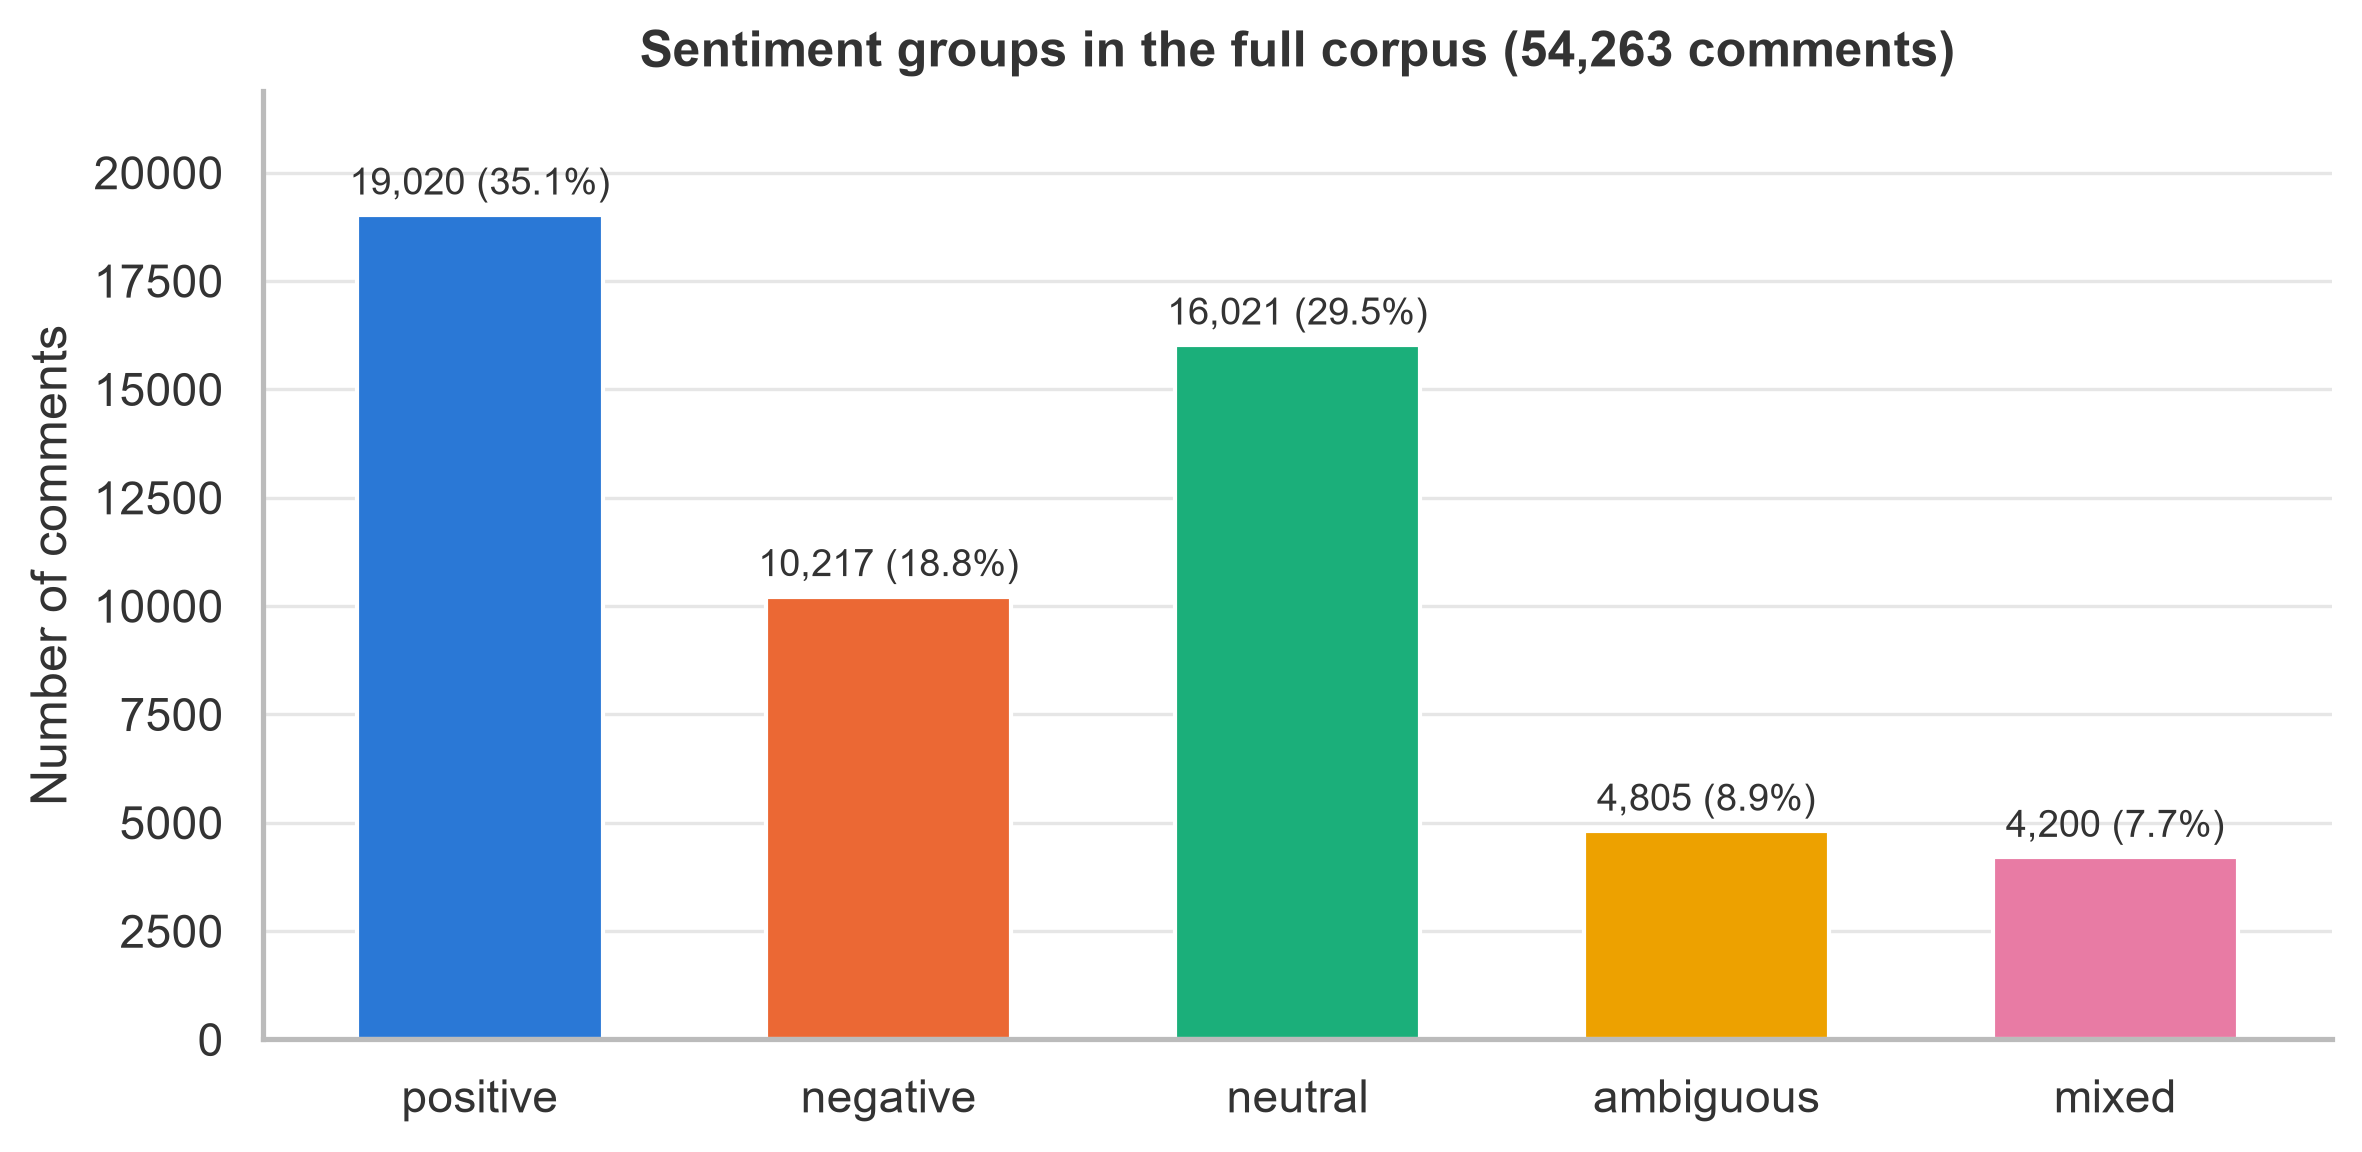
\includegraphics[width=\columnwidth]{eda_sentiment_groups.png}
\caption{Sentiment groups in the 54,263 comments after applying the official mapping.
Positive comments are 1.9 times more frequent than negative ones.}
\label{fig:groups}
\end{figure}

\subsection{Deduplication, balancing and split}

Duplicates are removed before sampling, comparing texts after stripping and lowercasing. Among
the 29,237 positive/negative candidates, 213 exact copies are dropped (mostly short replies such
as ``thank you!''), and one text that appears with both labels (``Weird flex but ok'') is
removed with all its 3 copies, leaving 29,021 comments. From them, 500 positive and 500
negative comments are sampled with \texttt{SEED = 42}, so that the majority baseline is exactly
50\% accuracy. The 1,000 comments are split 80/20 with stratification into 800 training
(400/400) and 200 test comments (100/100), with no text shared between both sets. For
hyperparameter selection, 15\% of the training set (120 comments, stratified) is held out as
validation; the test set is never used to choose a model.

\subsection{Text cleaning}

Each comment is normalized as follows: apostrophes are unified, the placeholders
\texttt{[NAME]} and \texttt{[RELIGION]} become the tokens \texttt{nametoken} and
\texttt{religiontoken}, URLs are removed, emojis are converted to word tokens with
\texttt{emoji.demojize} (e.g.\ \texttt{smiling\_face\_with\_heart\_eyes}), text is lowercased,
negative contractions are expanded (``don't'' $\rightarrow$ ``do not''), and punctuation and
digit-only tokens are removed. Finally the NLTK English stopwords \cite{bird2009natural} are removed
\emph{except negations}: 177 stopwords are dropped while negation words such as \texttt{not},
\texttt{no}, \texttt{nor} and \texttt{never} are kept. Removing negations would turn ``not happy'' into
``happy''. In the balanced set, \texttt{not} appears in 32.6\% of the negative comments and in
16.8\% of the positive ones, and it is the most frequent token of both classes
(Fig.~\ref{fig:unigrams}); with the full stopword list only 3.8\% and 1.8\% of the comments
would keep any negation word. Emojis are rare (25 comments of the balanced set) but are kept
because they carry sentiment.

After cleaning, comments have 6.98 tokens on average (13.05 words before cleaning), the 95th
percentile is 13 and the longest has 20 tokens. We therefore use sequences of length
\texttt{MAX\_LEN = 30}, which truncates no comment; 76.8\% of the positions of the training
matrix are padding.

\begin{figure}[t]
\centering
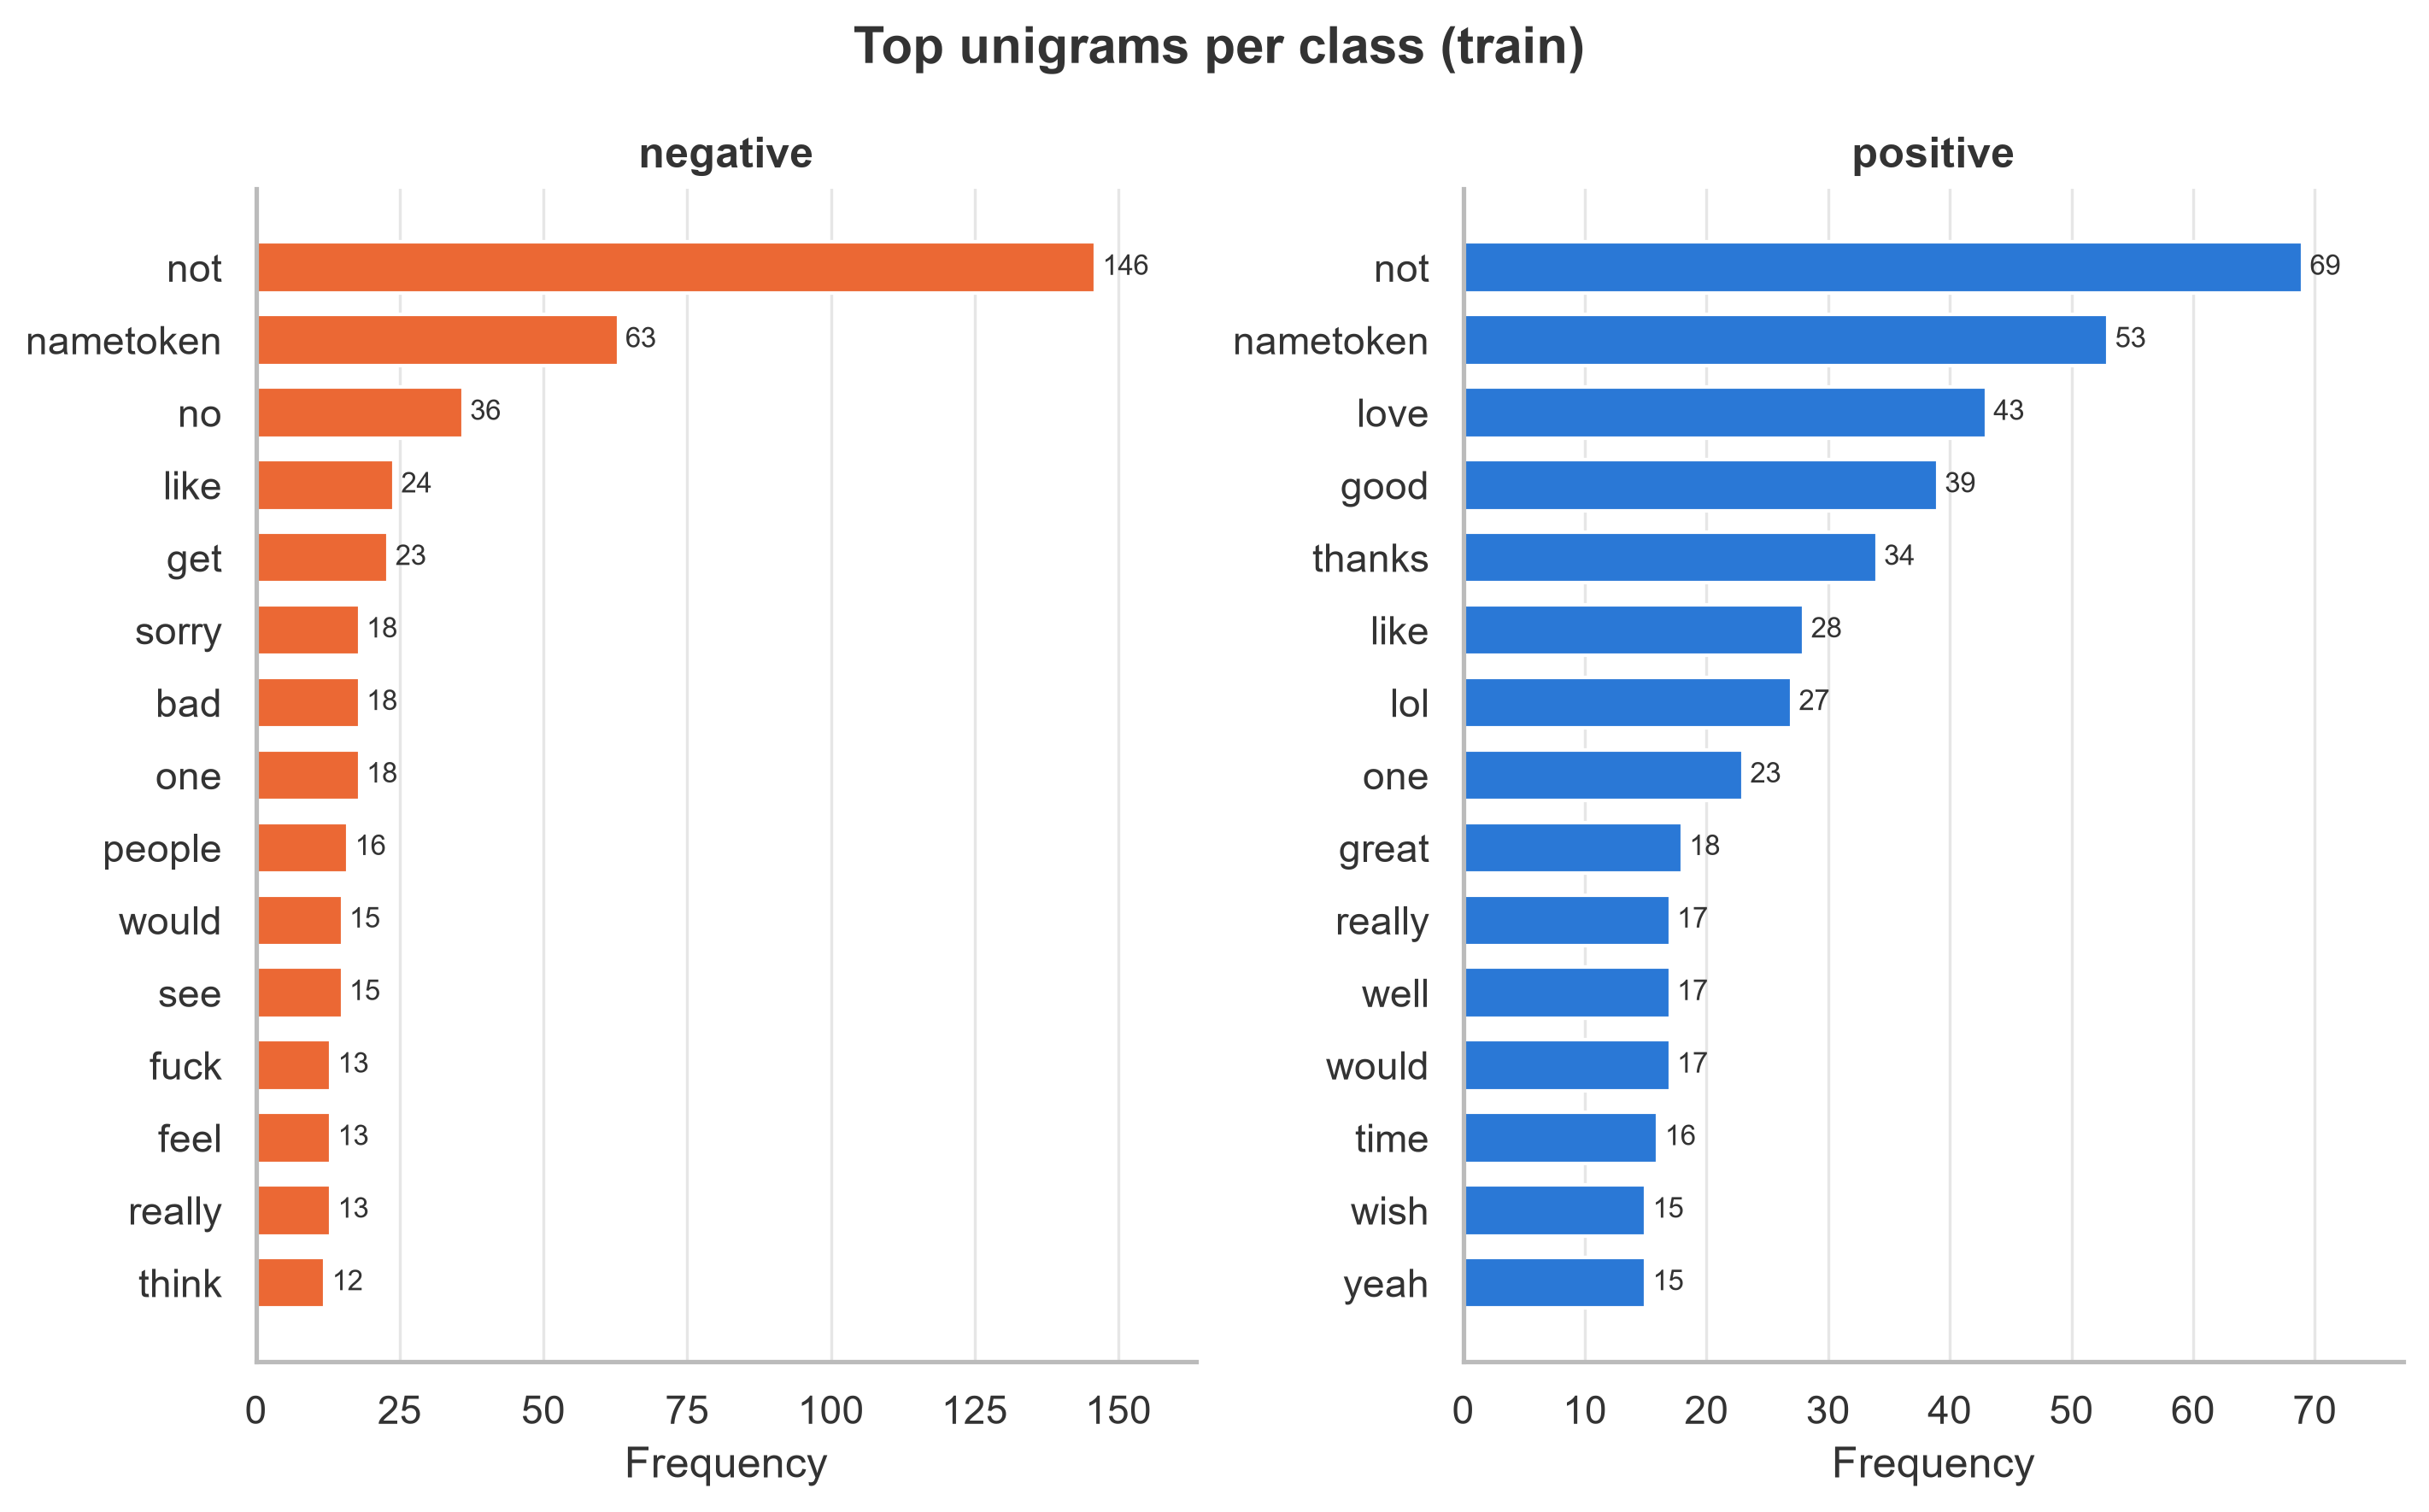
\includegraphics[width=\columnwidth]{eda_top_unigrams.png}
\caption{Most frequent tokens per class in the training set after cleaning. The negation
\texttt{not} is kept and is twice as frequent in negative comments.}
\label{fig:unigrams}
\end{figure}

\subsection{Vectorization}

The Dense, RNN and LSTM models share the same input: a Keras \texttt{TextVectorization}
layer that splits the cleaned text on whitespace and maps every token to an integer, padded to
30 positions. The layer is adapted \emph{only on the training texts}, so no information
from the test set leaks into the features. The vocabulary has 2,364 tokens (2,366 ids with
padding and the unknown token), and 67.6\% of them appear only once. As a consequence, 30.7\% of
the test tokens are out of vocabulary and 162 of the 200 test comments contain at least one
unknown word; the validation split shows a similar rate (28.2\%), so it is a realistic proxy
for the test condition. This sparsity is expected with 800 short comments and is one of the
motivations for the pre-trained Transformer of Section~\ref{sec:transformer}, which uses its
own subword tokenizer on the raw text.

\section{Models and Training}
\label{sec:models}

Each neural classifier learns a token embedding, ignores padding, and applies
dropout to the comment representation before a single sigmoid output. Dense
averages the token embeddings and passes the mean through a ReLU layer. Thus,
reordering the same tokens leaves its prediction unchanged. The recurrent
models instead read tokens in order and classify the final hidden state.

Let $x_t$ denote the embedding at position $t$. SimpleRNN~\cite{elman1990finding}
updates $h_t=\tanh(Wx_t+Uh_{t-1}+b)$. The LSTM~\cite{hochreiter1997long}
also maintains a cell state $c_t$. Writing $z_t=[x_t;h_{t-1}]$ and
$a_j=W_jz_t+b_j$, its update is
\begin{gather*}
 i_t=\sigma(a_i),\quad f_t=\sigma(a_f),\quad o_t=\sigma(a_o),\\
 g_t=\tanh(a_g),\qquad c_t=f_t\odot c_{t-1}+i_t\odot g_t,\\
 h_t=o_t\odot\tanh(c_t).
\end{gather*}
The forget gate $f_t$ controls how much of the previous cell state survives,
the input gate $i_t$ scales the candidate update $g_t$, and the output gate
$o_t$ controls how much of the cell state enters $h_t$.

For each architecture we tested 48 combinations: embedding dimension
$d\in\{32,64\}$, hidden units $h\in\{16,32,64\}$, dropout
$p\in\{0.2,0.5\}$, Adam learning rate $\eta\in\{0.001,0.003\}$, and batch
size $B\in\{16,32\}$. With seed 42, we fit on 680 comments for up to 30 epochs
using binary cross-entropy. Early stopping restored the lowest validation
loss after three epochs without improvement. We ranked configurations by
macro F1 on the same 120 validation comments, breaking ties by lower loss.

\begin{table}[t]
\caption{Validation winners and parameter counts after full-training refit.}
\label{tab:neural-config}
\centering\footnotesize
\begin{tabular}{@{}lrrrrrrr@{}}
\toprule
Model & $d$ & $h$ & $p$ & $\eta$ & $B$ & Val.\ F1$_m$ & Params.\\
\midrule
Dense & 32 & 32 & .5 & .003 & 32 & .758 & 76,801\\
SimpleRNN & 32 & 64 & .5 & .001 & 16 & .628 & 81,985\\
LSTM & 64 & 32 & .5 & .003 & 32 & .733 & 163,873\\
\bottomrule
\end{tabular}
\end{table}

For each winner in Table~\ref{tab:neural-config}, we selected the epoch count
separately for seeds 42--46 using the same validation split. We then refit each
seed from scratch on all 800 training comments for that count. Vocabulary size
grew from 2,138 IDs during tuning to 2,366 for the final fits. We selected one
seed per architecture for export using validation macro F1, with lower loss
and then lower seed as tie-breakers.

\section{Evaluation and Results}
\label{sec:evaluation}

Among the five models, DistilBERT achieved the highest mean test macro F1
(0.843), followed by Dense (0.741), LSTM (0.701), SimpleRNN (0.551), and
the stratified dummy (0.516). Table~\ref{tab:neural-results} reports five
seeds for the dummy and recurrent models and three for DistilBERT. The
positive-class metrics use label 1; macro F1 weights both classes equally.

\begin{table*}[t]
\caption{Training and held-out test performance. Entries are mean $\pm$
sample standard deviation on one fixed split (five seeds except DistilBERT,
which used three).}
\label{tab:neural-results}
\centering\footnotesize
\begin{tabular}{@{}llrrrrrr@{}}
\toprule
Split & Model & Accuracy & Precision & Recall & F1 & Macro F1 & Cohen's $\kappa$\\
\midrule
Train & Dummy & $0.498\pm0.027$ & $0.497\pm0.026$ & $0.500\pm0.046$ & $0.498\pm0.036$ & $0.498\pm0.027$ & $-0.004\pm0.054$\\
Train & Dense & $0.990\pm0.006$ & $0.990\pm0.012$ & $0.990\pm0.006$ & $0.990\pm0.006$ & $0.990\pm0.006$ & $0.980\pm0.013$\\
Train & SimpleRNN & $0.816\pm0.101$ & $0.856\pm0.047$ & $0.757\pm0.208$ & $0.792\pm0.139$ & $0.812\pm0.107$ & $0.632\pm0.202$\\
Train & LSTM & $0.946\pm0.041$ & $0.975\pm0.016$ & $0.915\pm0.086$ & $0.942\pm0.047$ & $0.945\pm0.041$ & $0.891\pm0.081$\\
\midrule
Test & Dummy & $0.517\pm0.025$ & $0.516\pm0.024$ & $0.540\pm0.039$ & $0.528\pm0.028$ & $0.516\pm0.025$ & $0.034\pm0.050$\\
Test & Dense & $0.744\pm0.038$ & $0.727\pm0.065$ & $0.802\pm0.059$ & $0.759\pm0.018$ & $0.741\pm0.043$ & $0.488\pm0.077$\\
Test & SimpleRNN & $0.563\pm0.036$ & $0.562\pm0.030$ & $0.530\pm0.208$ & $0.531\pm0.126$ & $0.551\pm0.047$ & $0.126\pm0.072$\\
Test & LSTM & $0.704\pm0.020$ & $0.712\pm0.066$ & $0.714\pm0.109$ & $0.704\pm0.032$ & $0.701\pm0.021$ & $0.408\pm0.040$\\
Train & DistilBERT & $0.936\pm0.001$ & $0.951\pm0.007$ & $0.919\pm0.006$ & $0.9347\pm0.0004$ & $0.9358\pm0.0008$ & $0.872\pm0.002$\\
Test & DistilBERT & $0.843\pm0.006$ & $0.868\pm0.021$ & $0.810\pm0.017$ & $0.838\pm0.004$ & $0.843\pm0.006$ & $0.687\pm0.012$\\
\bottomrule
\end{tabular}
\end{table*}

DistilBERT achieved the highest test macro F1 (0.843 $\pm$ 0.006) and
accuracy (0.843 $\pm$ 0.006); its mean train-to-test macro-F1 gap was 0.093.
Dense was the strongest of the non-Transformer models, but its larger
train-to-test gap (0.249) indicates more overfitting. DistilBERT's three
seeds and the other models' five seeds were evaluated on the same 200 test
comments, so these standard deviations describe run variation, not sampling
uncertainty.

\begin{table}[t]
\caption{Test confusion matrices for the validation-selected checkpoints.
Each pair gives predictions (negative, positive) for one true class;
each true class contains 100 comments.}
\label{tab:neural-confusion}
\centering\footnotesize
\begin{tabular}{@{}lrrr@{}}
\toprule
Model & Seed & True negative class & True positive class\\
\midrule
Dense & 42 & (75, 25) & (20, 80)\\
SimpleRNN & 46 & (39, 61) & (21, 79)\\
LSTM & 42 & (77, 23) & (34, 66)\\
\bottomrule
\end{tabular}
\end{table}

Table~\ref{tab:neural-confusion} shows why the recurrent models differ.
LSTM reduced false positives from 61 to 23 relative to SimpleRNN, but
missed 34 positive comments versus 21. On the positive comment
\emph{I didn't find it too bad}, SimpleRNN recovered the approval label and
LSTM predicted negative. Both models missed a negative comment that used
\emph{good} in an apparently ironic question. Cleaning retained the word
and removed its quotation marks.

\section{Transformer Extension}
\label{sec:transformer}

% To be completed

\section{Model Comparison and Relation to Turing Machines}
\label{sec:comparison}

The fixed 200-comment test split ranks mean macro F1 as DistilBERT (0.843
$\pm$ 0.006), Dense (0.741 $\pm$ 0.043), LSTM (0.701 $\pm$ 0.021),
SimpleRNN (0.551 $\pm$ 0.047), then the stratified dummy (0.516 $\pm$ 0.025).
The train/test gaps are 0.093 for DistilBERT and 0.249 for Dense. Standard
deviations describe run variation on this split; DistilBERT used three seeds
and the other models used five.

Final-refit CPU times exclude hyperparameter search: Dense, SimpleRNN and LSTM
took about 0.9--1.5 s, while DistilBERT averaged 10.7 min with high variation.
Inference on 1,000 tokenized comments took 47.19 s for DistilBERT and
0.18--0.22 s for the smaller neural models. These hardware-dependent timings
exclude text cleaning and tokenization. Table~\ref{tab:model-cost} reports the
fit, inference and parameter measurements.

For length $T$, embedding width $d$ and hidden width $h$, Dense mean-pooling
costs $O(Td)$, SimpleRNN costs $O(T(dh+h^2))$ sequential operations, and LSTM
has the same order with a larger gate-related constant. DistilBERT's parallel
self-attention costs $O(T^2d)$ per layer. These terms describe sequence
operations, not full wall-clock time.

\begin{table}[t]
\caption{Mean final-fit time, parameter count, and CPU inference time. Fit time is mean $\pm$ sample SD across five runs, or three for DistilBERT; it excludes hyperparameter search.}
\label{tab:model-cost}
\centering\scriptsize
\setlength{\tabcolsep}{2pt}
\begin{tabular}{@{}lrrr@{}}
\toprule
Model & Fit (s) & Params. & Infer./1,000 (s)\\
\midrule
Dummy & $<0.001$ & 0 & 0.0005\\
Dense & $0.86\pm0.06$ & 76,801 & 0.184\\
SimpleRNN & $1.30\pm0.11$ & 81,985 & 0.185\\
LSTM & $1.51\pm0.12$ & 163,873 & 0.221\\
DistilBERT & $644.9\pm424.1$ & 66.96M & 47.193\\
\bottomrule
\end{tabular}
\end{table}

Interpretability varies: Dummy's rule is transparent but text-blind; Dense
averages inspectable token vectors but loses order; RNN/LSTM hide decisions in
learned states. DistilBERT attention is inspectable, not causal.

Turing-completeness results for recurrent networks and Transformers require
idealized assumptions~\cite{siegelmann1995computational,perez2021attention}.
These trained models have fixed parameters, finite precision and bounded inputs,
so every inference terminates. The positive-comment label is a statistical
target, not a formal language; irony and missing context limit this experiment.

\section{Conclusions}
\label{sec:conclusions}

% To be completed


\bibliographystyle{IEEEtran}
\bibliography{../references}

\end{document}
